\documentclass[a4paper]{article}

\usepackage{amsthm}
\newtheorem{theorem}{Twierdzenie}[section]
\theoremstyle{definition}
\newtheorem{zadanie}[theorem]{Zadanie}
\newtheorem{definicja}[theorem]{Definicja}

\usepackage{graphicx}
\graphicspath{ {./} }
\usepackage{xcolor}
\usepackage{listings}
\usepackage{tikz}
\usetikzlibrary{matrix}
\graphicspath{ {./} }
\definecolor{codegreen}{rgb}{0,0.6,0}
\definecolor{codegray}{rgb}{0.5,0.5,0.5}
\definecolor{codepurple}{rgb}{0.58,0,0.82}
\definecolor{backcolour}{rgb}{0.95,0.95,0.92}
\lstdefinestyle{mystyle}{
    backgroundcolor=\color{backcolour},   
    commentstyle=\color{codegreen},
    keywordstyle=\color{magenta},
    numberstyle=\tiny\color{codegray},
    stringstyle=\color{codepurple},
    basicstyle=\ttfamily\footnotesize,
    breakatwhitespace=false,         
    breaklines=true,                 
    captionpos=b,                    
    keepspaces=true,                 
    numbers=left,                    
    numbersep=5pt,                  
    showspaces=false,                
    showstringspaces=false,
    showtabs=false,                  
    tabsize=2
}

\lstset{style=mystyle}

\usepackage[hmargin=1.5cm,vmargin=1.5cm]{geometry}

\usepackage{polski}
\usepackage[utf8]{inputenc}

\usepackage{hyperref}
\hypersetup{colorlinks=true,linkcolor=blue}

\title{Nauka C\#}
\author{Krystian Gronkowski}
\date{\today}

\begin{document}

\tikzset{ 
    table/.style={
        matrix of nodes,
        row sep=-\pgflinewidth,
        column sep=-\pgflinewidth,
        nodes={
            rectangle,
            draw=black,
            align=center
        },
        minimum height=1.5em,
        text depth=0.5ex,
        text height=2ex,
        nodes in empty cells,
%%
        every even column/.style={
            nodes={fill=gray!20}
        }
    }
}

\maketitle
\tableofcontents
	
\pagebreak
\section{Hello, world!}
\subsection{Konfigurowanie kompilatora}
Zanim zaczniemy programować musimy zaintalować kompilator, aby być w stanie otworzyć program który napiszemy.
\\\\W Linuxie kompilator mcs można zainstalować za pomocą komend:
\\\\sudo apt-get update
\\sudo apt-get install mono-mcs
\\\\Natomiast w Windowsie należy najpierw zainstalować .NET Framework, a potem dodać ścieżkę instalacji w zmiennej środowiskowej "PATH"
\\\\Alternatywnie, jeżeli ktoś nie chce instalować kompilatora, można użyć jednego z wielu edytorów C\# online, np: \url{https://www.onlinegdb.com/online_csharp_compiler}
\subsection{Console.WriteLine i Console.Readline}
Nadszedł czas na stworzenie pierwszego programu!
\\Struktura piku źródłowego C\# wygląda następująco:
\lstset{language=C}
\begin{lstlisting}[frame=single]
using System;

class NazwaPliku {
  static void Main() {
    //Kod
  }
}
\end{lstlisting}
\\	\\\textbf{Console.WriteLine()} jest funkcją wyświetlającą tekst na ekranie (jak printf w języku C), a \textbf{Console.ReadLine()} jest używany do wczytywania tekstu z klawiatury (jak scanf).
\\Przykładowy program wykorzystujący te dwie funkcje aby wyświetlić imie użytkownika na ekranie:
\lstset{language=C}
\begin{lstlisting}[frame=single]
using System;

public class HelloWorld
{
    public static void Main()
    {
        Console.WriteLine("Jak sie nazywasz?");
        string imie = Console.ReadLine();
        Console.WriteLine ("Witaj, "+imie+"!");
    }
}
\end{lstlisting}
\subsection{Konwersja danych}
Należy wziąć pod uwagę, że \textbf{Console.ReadLine()} zawsze wczytuje wartość string, gdybyśmy chcieli aby program wczytywał liczbę zamiast imienia, musielibyśmy przekonwertować string do wartości int.\\
Na szczęście jest do tego wbudowana funkcja \textbf{Int32.Parse(string)}. Przykład jej użycia:\\
\begin{lstlisting}[frame=single]
using System;

public class HelloWorld
{
    public static void Main(string[] args)
    {
        Console.WriteLine("Ile masz lat?");
        int wiek = Int32.Parse(Console.ReadLine());
	      if(wiek>17){
        	  Console.WriteLine("Jestes pelnoletni");
	      }
	      else{
		        Console.WriteLine("Nie jestes pelnoletni");
	      }
    }
}
\end{lstlisting}
\section{Pętle}
C\# zawiera wiele rodzaji pętli. Wszystkie z nich są przedstawione poniżej. Większość z nich jest wam zapewnie dobrze znana, ale zwróćcie szczególną uwagę na jedną specjalną do języka C\# - foreach.\\
\begin{lstlisting}[frame=single]
using System;

class Contains {
  static void Main() {
	int tablica[10] = new int[10];
	//Petla for
  for(int x=0;x<10;x++){
		Console.WriteLine(tablica[x]);
	}
	
	//Petla while
	int x = 0;
	while(x<10){
		Console.WriteLine(tablica[x]);
		x++;
	}

	//Petla foreach
	foreach(int x in tablica){
		Console.WriteLine(tablica[x]);
  }
}
\end{lstlisting}\\
\textbf{for} – pętla, którą zazwyczaj będziemy używać kiedy będziemy chcieli wykonać kod określoną ilość razy.\\\addvspace{5}
\textbf{while} – ta pętla ma prostszą budowę niż poprzednia ponieważ zawiera jedynie warunek wykonania. \\\addvspace{5}
\textbf{foreach} – ostatnia z omawianych pętli. W tym wypadku mamy specyficzny rodzaj pętli używany konkretnie do działania na kolejnych elementach wszelkiego rodzaju list, kolekcji itd.\\\addvspace{35}
\\Oprócz pętli potrzebnymi narzędziami są również instrukcje \textbf{if} oraz \textbf{else}. Działają one tak samo jak w C. Przykłady ich użycia są pokazane poniżej.\\
\begin{lstlisting}[frame=single]
using System;

class Contains {
  static void Main() {

	int x = 15;
	int y = 30;

	if(x+y>10){
		Console.WriteLine("x + y > 10");
	}
	else{
		Console.WriteLine("x + y < 10");
	}
}
\end{lstlisting}\\
\pagebreak
\section{Operowanie na danych}
\subsection{String.Contains}
\textbf{String.Contains()} jest bardzo użyteczną funkcją, która sprawdza czy gdziekolwiek w jakimś łańcuchu można znaleźć inny łańcuch. Zwraca wartość boolowską. Przykładem jego zastosowania jest sprawdzenie czy w jakimś słowie występuje litera 'a' :\\
\begin{lstlisting}[frame=single]
using System;

class Contains {
    static void Main() {
    	  Console.WriteLine("Wpisz slowo bez litery a");
        string x = Console.ReadLine();
        if(x.Contains('a')){
        	Console.WriteLine("W tym slowie jest litera a.");
        }
        else{
        	Console.WriteLine("W tym slowie nie ma litery a.");
        }
    }
}
\end{lstlisting}
\subsection{String.Replace}
\textbf{String.Replace()} zastępuje wszystkie wystąpienia łancucha A innym łańcuchem B.\\
\begin{lstlisting}[frame=single]
using System;

class Replace {
    static void Main() {
        string x = "Ala ma kota.";
        x = x.Replace("kota","psa");
        Console.WriteLine(x);
        // W konsoli zostanie wyswietlone "Ala ma psa."
    }
}
\end{lstlisting}
\subsection{String.Split}
\textbf{String.Split()} rozdziela łańcuch na tablicę mniejszych łańcuchów rozdzielonych za pomocą łańcucha podanego podczas wywoływania funkcji. Bardzo użyteczne jeżeli chcemy odczytać dane rozdzielone za pomocą nowej linijki albo spacji. Przykład użycia:\\
\begin{lstlisting}[frame=single]
using System;

class Split {
    static void Main() {
        Console.WriteLine("Wpisz swoje imie i nazwisko");
        string x = Console.Readline();
        string[] input = x.Split(' ');
        string imie = input[0];
        string nazwisko = input[1];
        Console.WriteLine("Dzien dobry, Pani/e " + nazwisko);
    }
}
\end{lstlisting}
\begin{zadanie}
\\Poproś użytkownika o wpisanie jakiegoś zdania, a potem wyświetl je ze słowami w odwrotnej kolejności.
\\\textrm{Ala ma kota \rightarrow \textrm{kota  ma  Ala}}
\end{zadanie}
\begin{zadanie}
\\Poproś użytkownika o wpisanie jakiegoś słowa i wyświetl wszystkie litery które w nim nie występują.
\end{zadanie}
\pagebreak
\section{Tablice i listy}
\subsection{Tablice jednowymiarowe}
Tablica to zbiór uporządkowanych elementów tego samego typu. Każdy element można wyczytać podając numer jego indeksu. Przykład zastosowania tablicy aby sprawdzić ile razy każda cyfra występuje w jakiejś liczbie.\\
\begin{lstlisting}[frame=single]
using System;

class HelloWorld {
    static void Main() {
    	int[] tablica = new int[10];
        string liczba = "1049284883920457162047859300018306";
        for(int i=0;i<liczba.Length;i++){
        	tablica[Int32.Parse(liczba[i].ToString())]+=1;
        }
        for(int i=0;i<10;i++){
        	Console.WriteLine("Liczba " + i + " wystepuje " + tablica[i] + " razy.");
        }
    }
}

\end{lstlisting}
\subsection{Tablice wielowymiarowe}
Najprostszy sposób patrzenia na tablice dwuwymiarową tablica[k][w] jest wyobrażenie sobie tabelki o k kolumnach i w wierszach.\\
Dla przykładu, popatrzmy na tablicę dwuwymiarową [5][3] wypełnioną w następujący sposób:
\\\\
\begin{tikzpicture}

\matrix (first) [table,text width=6em]
{
1 & 4 & 6 & 2 & 0\\
2 & 7 & 7 & 0 & 3\\
-15 & 55 & 26 & 0 & 330\\
};
\end{tikzpicture}\\
tablica[1][0] nawiązuje do liczby w 2 kolumnie i w 1 wierszu (pamiętaj że tablica zaczynają się od 0!), czyli do liczby 4. W ten sam sposób tablica[2][2] dałaby wynik 26, a tablica[0][0] 1.
\begin{zadanie}
\\Stwórz tablicę dwuwymiarową[10][10] i wypełnij ją tabliczką mnożenia.
\end{zadanie}
\subsection{Listy}
Listy działają jak tablice, ale nie mają zadeklarowanej wielkości. Można dodawać nowe elementy do listy i usuwać stare gdy tylko się chce. Jest to bardzo użyteczne, gdy chcemy przechować jakieś elementy, ale nie wiemy jak jest ich dużo. Na przykład gdy chcemy wczytywać liczby podawane przez użytkownika, dopóki nie wpisze 0.
\begin{lstlisting}[frame=single]
using System;
using System.Collections.Generic; //Biblioteka w ktorej znajduja sie listy

class HelloWorld {
    static void Main() {
        List<int> ints = new List<int>();
        while(true){
            int x = Int32.Parse(Console.ReadLine());
            if(x!=0){
                ints.Add(x);   
            }
            else{
                break;
            }
        }
        foreach(int x in ints){
            Console.WriteLine(x);
        }
    }
}
\end{lstlisting}
\pagebreak
\section{Losowanie liczb}

\textbf{new Random()} inicjalizuje nowy pseudolosowy generator liczb. W parametrze można podać ziarno według którego liczby mają się generować. W przypadku gdy w wywołaniu funkcji nie będą podane żadne parametry ziarno zostanie automatycznie ustawione jako czas otwarcia programu, w przeciwieństwie do C nie ma więc potrzeby ustawiania ziarna samodzielnie.
Aby otrzymać liczbę należy użyć polecenia \textbf{zmienna = random.Next(dolna granica, górna granica + 1)}.
\\Poniższy program inicjalizuje tablicę o wielkości 100 i wypełnia ją losowymi liczbami z zakresu 0-100:\\\begin{lstlisting}[frame=single]
using System;

public class Losowanie
{
    public static void Main()
    {
        int[] tablica = new int[100];
        Random r = new Random();
        for(int x=0;x<100;x++){
            tablica[x] = r.Next(0,101);
        }
        foreach(int i in tablica){
            Console.WriteLine(i);
        }
    }
}
\end{lstlisting}
\begin{zadanie}
\\System Martingale'a to system bukmacherski który polega na podwajaniu swojego zakładu za każdym razem gdy przegrasz grę w ruletkę. Ewentualna wygrana zwraca wszystkie poprzednie przegrane z bonusem orginalnego zakładu.
\\Czy ten system wydaje się dobrą strategią? Napisz program realizujący system Martingale'a i sprawdź jaką liczbę pieniędzy uda się wygrać komputerowi zanim straci swoje oszczędności jeżeli zacznie z 1000 zł i orginalna stawka będzie wynosić 5 zł tak jak w diagramie bloczkowym:
\\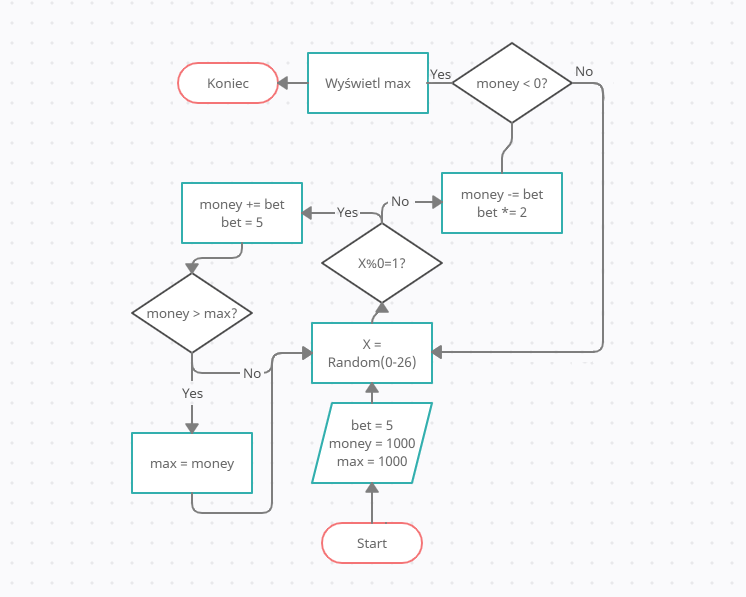
\includegraphics[scale=0.85]{bloczki}
\end{zadanie}
\pagebreak
\section{Operacje na plikach tekstowych}
\subsection{Wczytywanie plików}
Dane z plików tekstowych można wczytywać na różne sposoby - wszystko naraz do jednego łańcucha, do tablicy łańcuchów w której każdy indeks jest jednym wierszem pliku, lub można je wczytywać linijka po linijce. Wszystkie z tych sposobów zostały przedstawione poniżej:\\ 
\begin{lstlisting}[frame=single]
using System;

public class CzytaniePlikow
{
    public static void Main()
    {
    	//Caly plik zostal wczytany do linijki text.
   	 string text = System.IO.File.ReadAllText("\\Text.txt");
   	 
   	 //Plik zostaje podzielony na wiersze i wczytany do tablicy lancuchow.
   	 string[] lines = System.IO.File.ReadAllLines("\\Text.txt");
   	 
   	 foreach(line x in System.IO.File.ReadAllText("\\Text.txt")){
   	 	//Wczytuje linia po linijce w petli
   	 	Console.WriteLine(line);
   	 }
    }
}
\end{lstlisting}
\begin{zadanie}
W repozytorium znajduje się plik liczby.txt który jest wypełniony liczbami z przedziału [-100 ; 100], wczytaj z niego wszystkie liczby i oblicz ich średnią arytmetyczną oraz sumę.
\end{zadanie}
\subsection{Edycja plików tekstowych}
Biblioteka System.IO zawiera nie tylko funkcje do wczytywania plików tekstowych ale i do tworzenia i edycji plików. Służy do tego funkcja \textbf{System.IO.File.WriteAllText()}. Oto przykład jej zastosowania:\\
\begin{lstlisting}[frame=single]
using System;

public class EdycjaPLikow
{
    public static void Main()
    {
    	 string zawartosc = "Hello World!";
		   System.IO.File.WriteAllText("\\Text.txt", zawartosc); //Wypelni plik Text.txt lancuchem zawartosc
	
		   Console.WriteLine(System.IO.File.ReadAllText("\\Text.txt")); //Wyswietli zawartosc pliku Text
    }
}
\end{lstlisting}
\begin{thebibliography}{9}
\bibitem{texbook}
\url{https://automatykanacodzien.pl/2020/07/24/kompilacja-i-uruchomienie-kodu-c-w-linii-polecen-windows-linux/}
\bibitem{texbook2}
\url{https://pl.wikipedia.org/wiki/Tablica_(informatyka)}
\bibitem{texbook4}
\url{https://zajacmarek.com/2016/04/kurs-c-cz-7-petle/}
\bibitem{texbook3}
\url{https://en.wikipedia.org/wiki/Martingale_(betting_system)}
\bibitem{texbook3}
\url{https://docs.microsoft.com/pl-pl/dotnet/csharp/programming-guide/file-system/how-to-read-from-a-text-file}
\end{document}
